\chapter{Fundamental Geometry}

\section{Fundamental 01}

A \textbf{Segment} (đoạn thẳng) $\overline{AB}$ has finite length.

A \textbf{Line} (đường thẳng) $\overleftrightarrow{AB}$ extends out indefinitely in both directions.

A \textbf{Ray} (tia) $\overrightarrow{AB}$ only extends in one direction

A \textbf{Plane} (mặt phẳng) $ABC$

The \textbf{intersection} of two lines is a \textbf{point} (một điểm).

The \textbf{intersection} of two planes is a line.

\textbf{Collinear points} are points that lie on the same straight line.

\textbf{Coplanar points} are points that all lie on the same plane. Any two points are always coplanar, and any three points are always coplanar, even if they are collinear (on the same line). However, four or more points are coplanar only if they all lie on the same plane

\textbf{Opposite rays} (tia đối) are two rays that share the same endpoint and extend in exactly opposite directions. Together, they form a straight line.

\begin{figure}[ht]
  \centering
  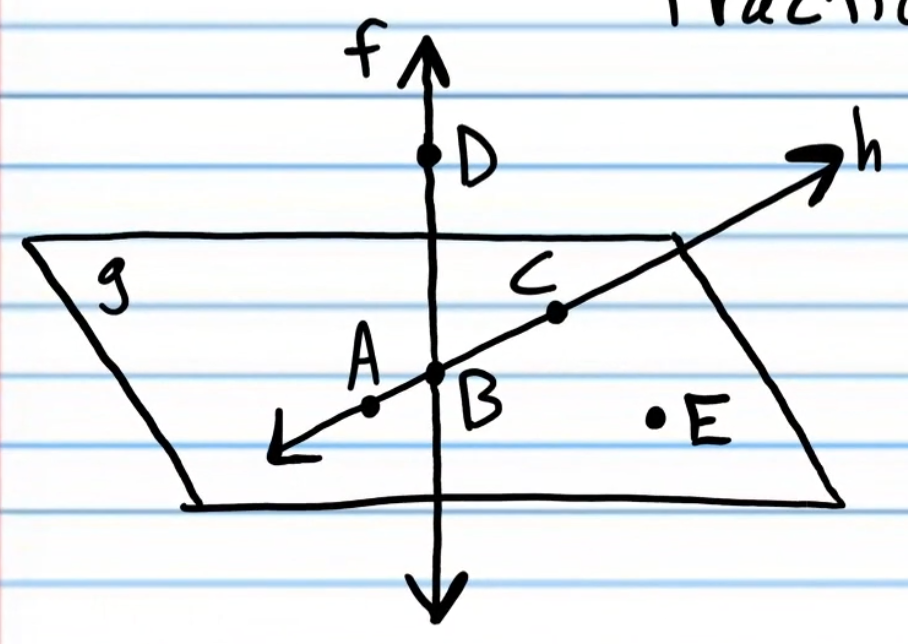
\includegraphics[width=0.5\textwidth]{0201.png}
  % \caption{fig 0201}
\end{figure}

Name three collinear points on the figure above: A, B and C

Name four coplanar points: A, B, C and E
